\documentclass[sigconf]{acmart}

\usepackage{graphicx}
\usepackage{amsmath}
\usepackage{enumitem}
\usepackage{float}
\usepackage[hidelinks]{hyperref}
\usepackage{placeins}

\settopmatter{printacmref=false}
\renewcommand\footnotetextcopyrightpermission[1]{}
\pagestyle{plain}

\title{Persistent One-Sided Order Books from Learned Trading Behavior}
\author{Jean-Paul Vestjens \\ \texttt{vestjejj@rose-hulman.edu}}
\date{}

\begin{document}

\begin{abstract}
This paper studies how increasing the participation of reinforcement learning (RL) trading agents affects liquidity in a limit order book. Using an agent-based market simulation, I vary the fraction of reinforcement learning agents and observe a nonlinear increase in persistent one-sided order book states, where either the best bid or best ask disappears and the mid-price becomes undefined.

I show that these failures tend to emerge in regimes where these agents remain active, not solely driven by trivial policy collapse into inactivity. A targeted anti-degeneracy intervention reduces extreme inactivity but does not remove the one-sided states. This suggests that the effect is driven by broader changes in agent behavior than by simple inactivity.

I further find that inventory constraints significantly reduce both the frequency and persistence of these one-sided order book states, restoring more stable two-sided liquidity. I also evaluate a mixed setting in which reinforcement learning participation is split between directional traders and passive quoting traders. This reduces the severity of one-sided order book failures but does not eliminate them, indicating that the failure is not explained solely by the absence of passive liquidity. Together, these results identify a failure mode in which learned trading behavior degrades liquidity and show that simple structural constraints can mitigate the impact.
\end{abstract}

\maketitle

\section{Introduction}

Financial markets rely on continuous two-sided liquidity, where both buy and sell orders are present in the limit order book. The availability of both sides is what allows prices to form through matching and keep spreads finite. When liquidity disappears from one side of the book, price formation breaks down and standard measures such as mid-price and spreads therefore become undefined. Understanding how such failures emerge is a central problem in market microstructure.

This paper shows that increasing the participation of reinforcement learning agents can produce a nonlinear rise in persistent one-sided order book states. These failures are strongest at intermediate values of $\phi$, persist even when a portion of RL agents provide passive liquidity, and are substantially mitigated by inventory constraints. This matters because it suggests that learned trading behavior can degrade market structure at the level of price formation itself rather than only through downstream measures such as volatility or volume.

Recent work has increasingly explored the use of reinforcement learning (RL) in trading and market making tasks. RL agents have been shown to learn effective strategies for order placement, inventory control, and execution in limit order book (LOB) environments (Spooner et al., 2018; Nevmyvaka et al., 2006). Many of these approaches rely on historical market replay or assume negligible market impact, which limits their ability to capture system-level effects that arise when multiple adaptive agents interact (Spooner et al., 2018). As a result, while RL-based strategies can optimize individual performance, they do not typically address how learning behavior alters the overall market structure.

Prior work in agent-based modeling has shown that interactions between heterogeneous trading agents can generate endogenous market instability. Specifically, studies have shown that coordination effects such as herding can reduce matching, lower liquidity, and effectively one-sided order flow (Lussange et al., 2024). More broadly, both academic and policy-oriented work has emphasized that algorithmic trading systems may withdraw liquidity under stress, amplifying market instability (Farmer and Foley, 2009; Bank of England, 2020; IMF, 2023). These findings show that liquidity provision is not fixed, but instead emerges from agent behavior and can degrade under certain conditions.

Despite this, there is limited work that directly studies how learned trading behavior affects the presence of both sides of the limit order book itself, rather than downstream outcomes such as volatility or volume. In particular, it remains unclear whether increasing the participation of learning-based agents leads to persistent states in which one side of the book disappears completely, and how such failures relate to agent-level decision making and participation behavior.

An important modeling question is whether such failures depend on reinforcement learning agents acting purely as liquidity takers. In many simulation settings, RL agents primarily submit aggressive market orders, which raises the concern that observed liquidity breakdowns may be driven by the removal of passive liquidity provision rather than by learned behavior itself. To address this, I also consider a mixed setting in which reinforcement learning participation is split between directional traders and agents that actively submit passive limit quotes. This allows me to test whether one-sided order book failures persist when learning-based agents are able to both consume and provide liquidity.

In this paper, I study how increasing the fraction of reinforcement learning agents in a limit order book affects liquidity provision, participation patterns, and the overall market structure. Using an agent-based simulation, I vary the proportion of RL agents and measure the emergence, frequency, and persistence of one-sided order book states. I focus on failures at the top of the book, where the best bid or best ask is absent and price formation becomes undefined.

I show that increasing the fraction of RL agents produces a nonlinear rise in persistent one-sided states. Importantly, these failures occur even when agents remain active, showing that the effect is not driven by trivial inactivity. I further show that allowing a portion of RL agents to provide passive liquidity reduces the severity of these failures but does not eliminate them. This indicates that the breakdown is not solely driven by the absence of liquidity provision, but instead arises from how learned agents allocate and withdraw liquidity over time. I also show that inventory constraints can significantly reduce both the persistence and frequency of these failures, partially restoring two-sided liquidity.

These findings identify a mechanism through which learned trading behavior can degrade the market structure and highlight the importance of incorporating system-level constraints when designing learning-based trading agents.

\section{Methods / Environment Setup}

\subsection{Market Environment}

All experiments were conducted using the ABIDES-based market simulation (Byrd et al., 2020). The simulation used a frozen RMSC-style configuration that consists of 102 agents interacting through a central exchange within a discrete-event kernel. The ABIDES framework allows for realistic limit order book dynamics by modeling message-level interactions between agents and the exchange and has been widely used in studies of market microstructure and algorithmic trading.

The market includes a latent fundamental value generated by a Gaussian random-walk oracle. Agents observe and act based on market conditions but do not have direct access to the fundamental value.

In this baseline configuration ($\phi = 0$), the agent population consists of:
\begin{itemize}[leftmargin=1.5em]
    \item 80 noise traders
    \item 20 value traders
    \item 2 adaptive market makers
\end{itemize}

\subsection{Control Parameters: RL Participation}

The primary experimental control parameter is the fraction of reinforcement learning (RL) agents, denoted by $\phi$. Increasing $\phi$ replaces a portion of the noise traders with these RL agents, while keeping value traders and market makers fixed. This ensures that changes in market behavior can be attributed specifically to the introduction of learned agents rather than changes in the overall structure of the market.

The experiment is run on the following grid:
\[
\phi \in \{0.00, 0.05, 0.10, 0.20, 0.30, 0.40, 0.50\}.
\]

\subsection{Agent Roles and Liquidity Provision}

Liquidity in the market is provided by the non-RL agents through a mix of passive and active behaviors:
\begin{itemize}[leftmargin=1.5em]
    \item Noise traders submit near-touch limit orders
    \item Value traders combine aggressive market orders with passive limit orders
    \item Adaptive market makers continuously provide two-sided limit quotes
\end{itemize}

In the baseline configuration, RL agents do not directly place passive limit orders. Instead, they interact with the market through aggressive market orders, meaning they primarily consume liquidity rather than provide it. Alternative configurations that allow RL agents to submit passive limit orders are introduced below.

\subsection{RL Liquidity Provision Modes}

In addition to the baseline setting in which reinforcement learning agents act purely as liquidity takers, I consider alternative configurations that allow RL agents to provide passive liquidity.

Two RL liquidity modes are evaluated:
\begin{itemize}[leftmargin=1.5em]
    \item \textbf{Taker-only:} RL agents submit only aggressive market orders (buy, sell) or remain inactive (hold), and do not place limit orders.
    \item \textbf{Mixed:} RL participation is split between directional agents and quoting agents. In this setting, a fixed fraction of RL agents operate as takers, while the remaining agents submit passive limit orders at the top of the book.
\end{itemize}

In the mixed setting, the default configuration uses a 50/50 split between taker and quoter agents. Quoting agents place limit orders at the current best bid and best ask with fixed size, allowing them to provide two-sided liquidity while interacting with the evolving market state.

This design allows for a controlled comparison between purely liquidity-consuming agents and agents that both consume and provide liquidity, enabling the analysis of whether one-sided order book failures depend on the absence of passive liquidity provision.

\subsection{RL Action and State Space}

Each RL agent operates with a discrete action space consisting of three actions:
\begin{itemize}[leftmargin=1.5em]
    \item 0 = sell
    \item 1 = hold
    \item 2 = buy
\end{itemize}

A buy or sell action results in the submission of a market order of fixed size (default size of 1), while a hold action results in no orders being submitted.

The state vector includes:
\begin{itemize}[leftmargin=1.5em]
    \item A rolling window of recent log returns
    \item Current bid-ask spread
    \item Order book imbalance
    \item Current inventory
\end{itemize}

The return window has a default length of 10, so the final vector is of dimension 13.

\subsection{Reward Function}

Rewards are computed per decision step and reflect the changes in marked-to-market wealth adjusted for risk and behavior penalties.

The function is defined as:
\[
r_t = \Delta W_t - \lambda_q \cdot 100 \cdot q_t^2 - P_{\text{hold}} - P_{\text{anti-degeneracy}}
\]

Where:
\begin{itemize}[leftmargin=1.5em]
    \item $\Delta W_t$ is the change in marked-to-market wealth
    \item $q_t$ is the agent's inventory
    \item $\lambda_q$ controls the quadratic inventory penalty
    \item $P_{\text{hold}}$ is an optional penalty for remaining inactive
    \item $P_{\text{anti-degeneracy}}$ penalizes extended sequences of hold actions
\end{itemize}

Rewards are applied at each decision transition and at the terminal step of each episode.

\subsection{Inventory Constraints}

Inventory is tracked directly from each agent's holdings. When the inventory constraints are enabled, actions that would violate a predefined inventory cap are automatically converted into hold actions before order submission.

This prevents agents from exceeding position limits while leaving the remaining market dynamics unchanged, allowing inventory constraints to act as a controlled intervention on agent behavior.

\subsection{Anti-Degeneracy Intervention}

To prevent trivial policy collapse into inactivity, some experiments include an anti-degeneracy intervention based on consecutive hold actions.

A hold streak is defined as the number of consecutive timesteps in which an agent selects the hold action. After a configurable grace period, an increasing penalty is applied to discourage extended inactivity. This penalty is incorporated directly into the reward function.

\subsection{Definition of One-Sided Order Book States}

The primary failure mode studied in this work is the one-sided order book state.

A market state is considered one-sided when either the best bid or best ask is missing in the top-of-book snapshot. In the data, this means:
\begin{itemize}[leftmargin=1.5em]
    \item Missing bid or ask values are recorded as NaN
    \item Mid-price is undefined when either side is missing
    \item Spread is undefined when either side is missing
\end{itemize}

I distinguish between:
\begin{itemize}[leftmargin=1.5em]
    \item True one-sided states, where exactly one side is missing
    \item Fully empty states, where both sides are missing
\end{itemize}

This definition focuses directly on the structure of the order book rather than derived quantities like volatility or volume.

\subsection{Experiment Protocol}

I evaluate system behavior through a sweep over $\phi$-sweep experiments. For each value of $\phi$, simulations are run for multiple episodes with independent random seeds.

The main experimental configuration includes:
\begin{itemize}[leftmargin=1.5em]
    \item 50 episodes per $\phi$
    \item Evaluation seeds: 7, 8, 9
    \item Both greedy and stochastic policy evaluation modes
\end{itemize}

In addition to the baseline (no inventory constraints), I evaluate:
\begin{itemize}[leftmargin=1.5em]
    \item RL liquidity provision modes (taker-only and mixed configurations)
    \item Inventory-constrained settings (caps of 50 and 20 units)
    \item Trained RL policies versus random baseline policies
    \item Anti-degeneracy interventions
\end{itemize}

Results are aggregated across seeds and episodes, and metrics are computed on logged market data, including measures of one-sided order book frequency, persistence, and related market quality indicators. For the key metrics reported in the main text, results are averaged across runs and uncertainty is shown using confidence intervals or error bars where available.

\section{Results}

\subsection{Emergence of One-Sided Order Book States}

I first examine how the frequency of one-sided order book states changes as the proportion of RL agents ($\phi$) increases.

As shown in Figure~\ref{fig:one-sided-book}, the fraction of timesteps in which the order book is one-sided remains low for $\phi \leq 0.2$, but rises sharply once RL participation moves beyond this range. Rather than indicating a gradual degradation in market quality, this pattern suggests a threshold-like shift in market functioning, where liquidity consumption begins to overwhelm the system's ability to replenish resting orders. Figure~\ref{fig:undefined-midprice} shows that the fraction of undefined mid-price observations tracks the same pattern, indicating that these one-sided states correspond to genuine breakdowns in price formation rather than a secondary artifact of the measurement procedure.

\begin{figure}[htbp]
    \centering
    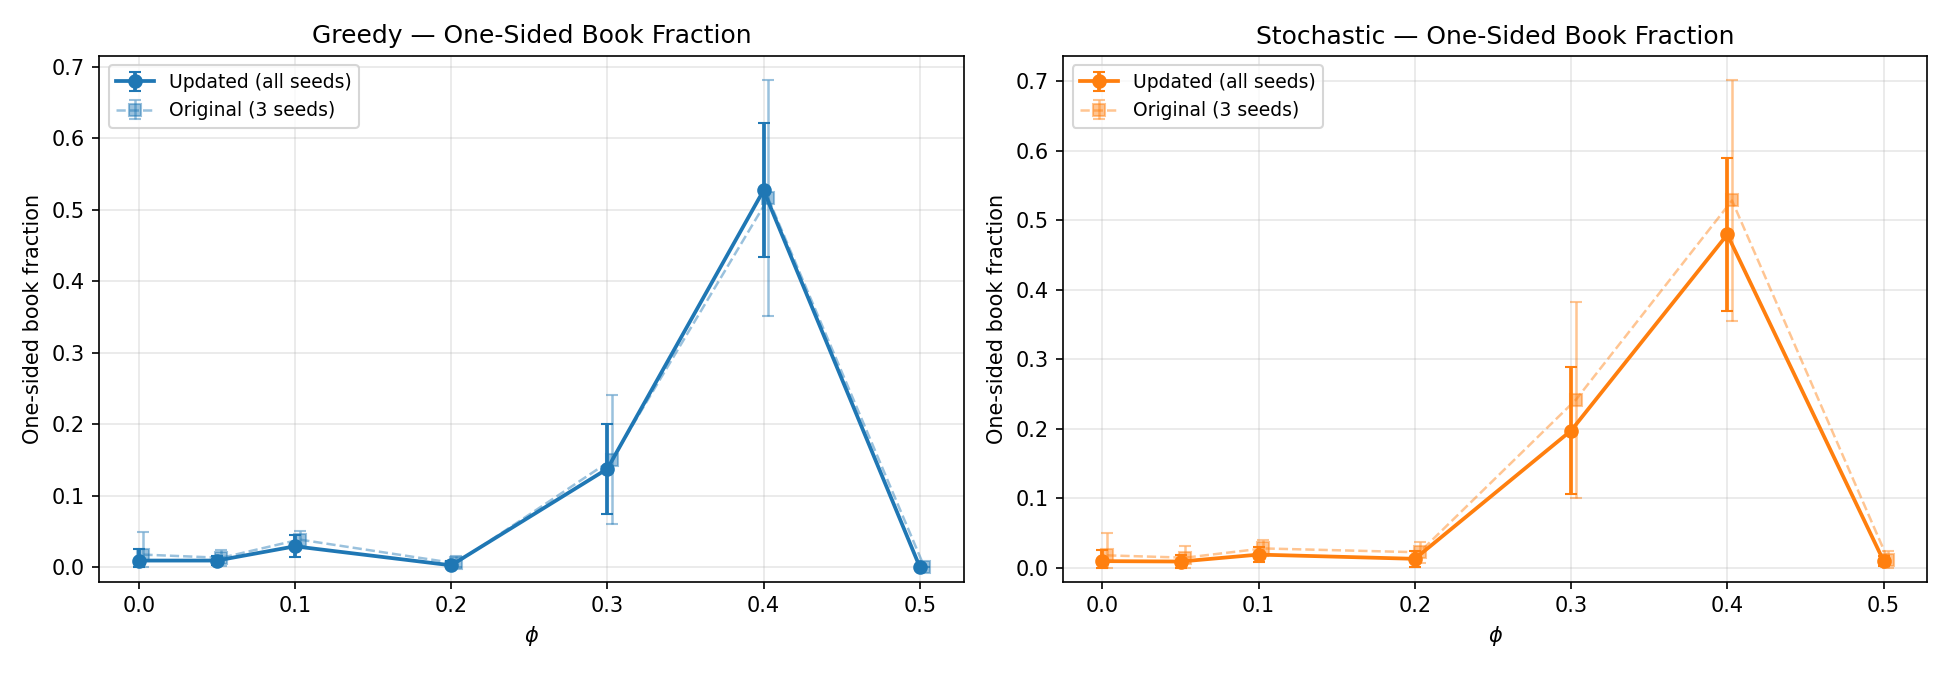
\includegraphics[width=\columnwidth]{updated_one_sided_fraction.png}
    \caption{One-Sided Order Book Fraction vs $\phi$. Fraction of timesteps in which the order book is one-sided, meaning either the best bid or best ask is missing, as a function of $\phi$ for both greedy and stochastic evaluation modes, with 95\% confidence intervals across six evaluation seeds.}
    \label{fig:one-sided-book}
\end{figure}

\begin{figure}[htbp]
    \centering
    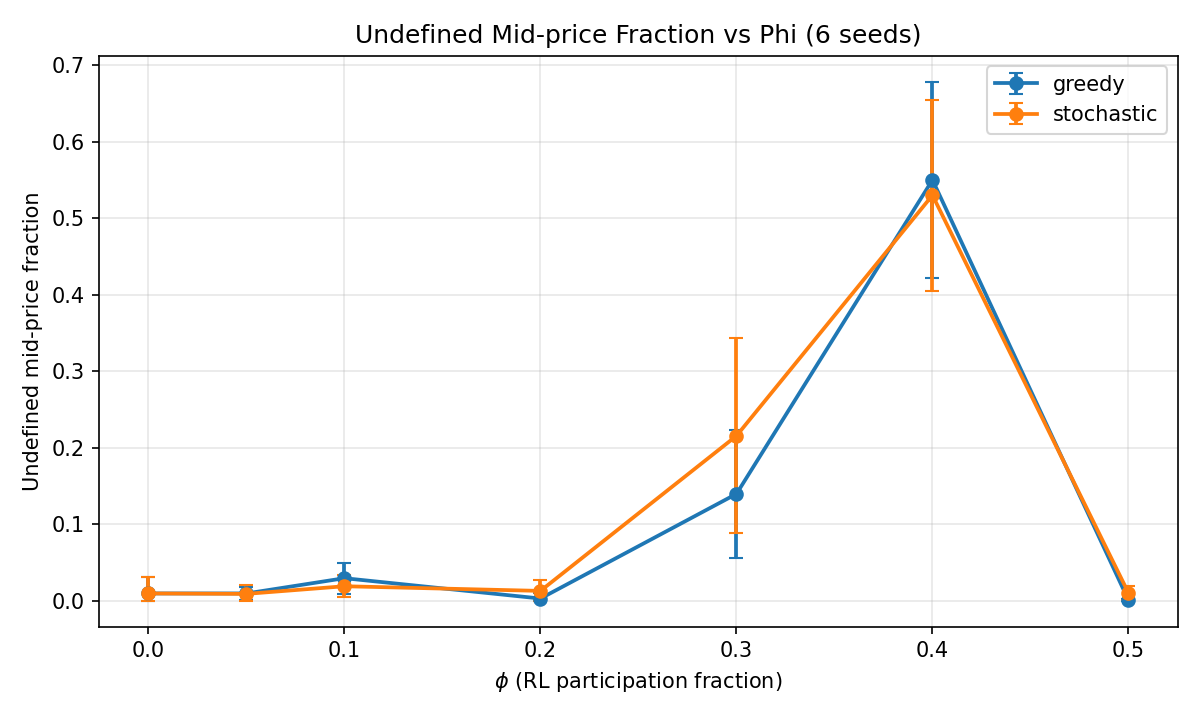
\includegraphics[width=\columnwidth]{undefined_midprice_fraction_with_ci_vs_phi.png}
    \caption{Undefined Mid-price Fraction vs $\phi$. Fraction of timesteps in which the mid-price is undefined due to the absence of either the best bid or best ask, with uncertainty shown across runs.}
    \label{fig:undefined-midprice}
\end{figure}

At $\phi = 0.5$, both metrics drop sharply. However, this does not reflect improved liquidity conditions. Instead, the system enters a degenerate near-shutdown regime in which market participation collapses.

\FloatBarrier

\subsection{Evidence That $\phi = 0.5$ Reflects Shutdown Rather Than Recovery}

To determine whether the drop in one-sided states at $\phi = 0.5$ reflects genuine recovery or market shutdown, I examine supporting behavioral and market-quality diagnostics.

As shown in Figure~\ref{fig:shutdown-support}, the drop in one-sided-book failures at $\phi = 0.5$ coincides with a sharp rise in inactivity, a sharp rise in zero-return behavior, and a collapse in quote activity. This combination indicates that the apparent improvement in one-sided-book metrics is not caused by healthier two-sided liquidity. Instead, it reflects a regime in which trading activity largely disappears. In this sense, $\phi = 0.5$ is better interpreted as a degenerate market state than as a recovery in market quality.

\begin{figure}[htbp]
    \centering
    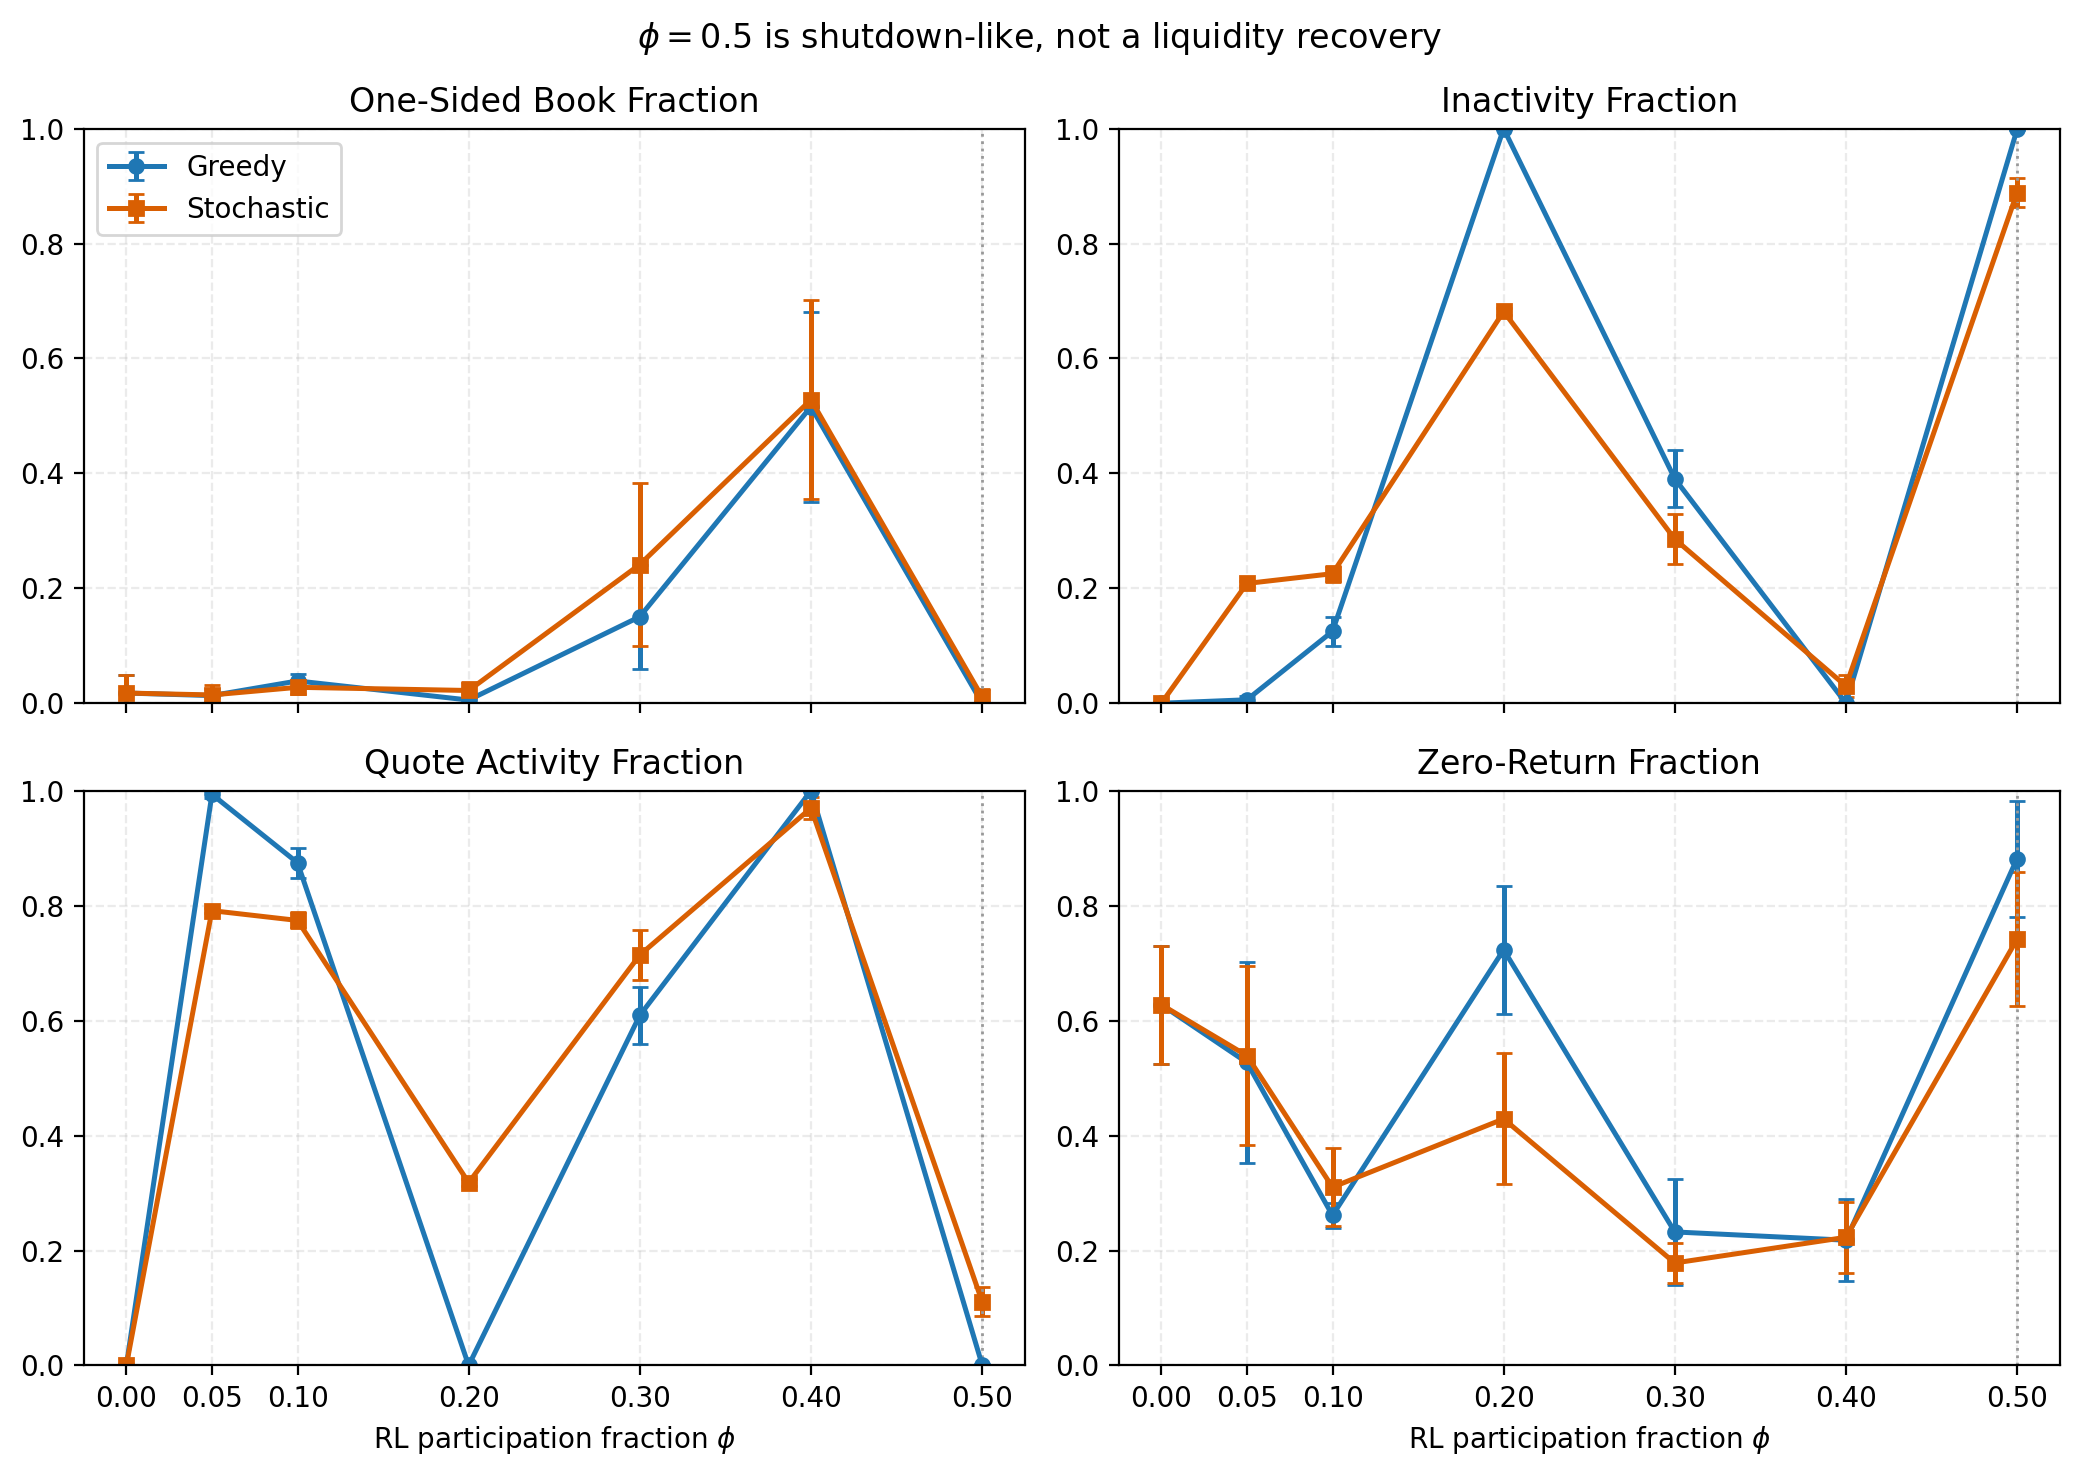
\includegraphics[width=\columnwidth]{phi_0_5_shutdown_support.png}
    \caption{Evidence that $\phi = 0.5$ is shutdown-like rather than a liquidity recovery. The drop in one-sided-book failures coincides with sharply higher inactivity, sharply higher zero-return behavior, and collapsed quote activity.}
    \label{fig:shutdown-support}
\end{figure}


\FloatBarrier

\subsection{Effects of RL Liquidity Provision Modes}

To determine whether one-sided order book failures depend on RL agents acting purely as liquidity takers, I compare taker-only and mixed liquidity configurations.

As shown in Figure~\ref{fig:liquidity-modes}, introducing passive quoting behavior reduces the frequency of one-sided order book states, particularly at intermediate values of $\phi$. In the mixed setting, where RL agents both consume and provide liquidity, the sharp nonlinear spike observed in the taker-only configuration is substantially dampened, particularly around $\phi = 0.3$ to $\phi = 0.4$.

This comparison matters because it rules out the simplest mechanical explanation for the baseline result. If one-sided failures were driven only by the removal of passive liquidity, then adding passive quotes back into the system should eliminate the effect. Instead, the mixed configuration remains more stable than the taker-only case but still exhibits elevated one-sided states relative to low-$\phi$ regimes. This indicates that passive liquidity alone is not sufficient to prevent breakdown. The instability also depends on how learning-based agents participate and withdraw liquidity over time.

\begin{figure}[htbp]
    \centering
    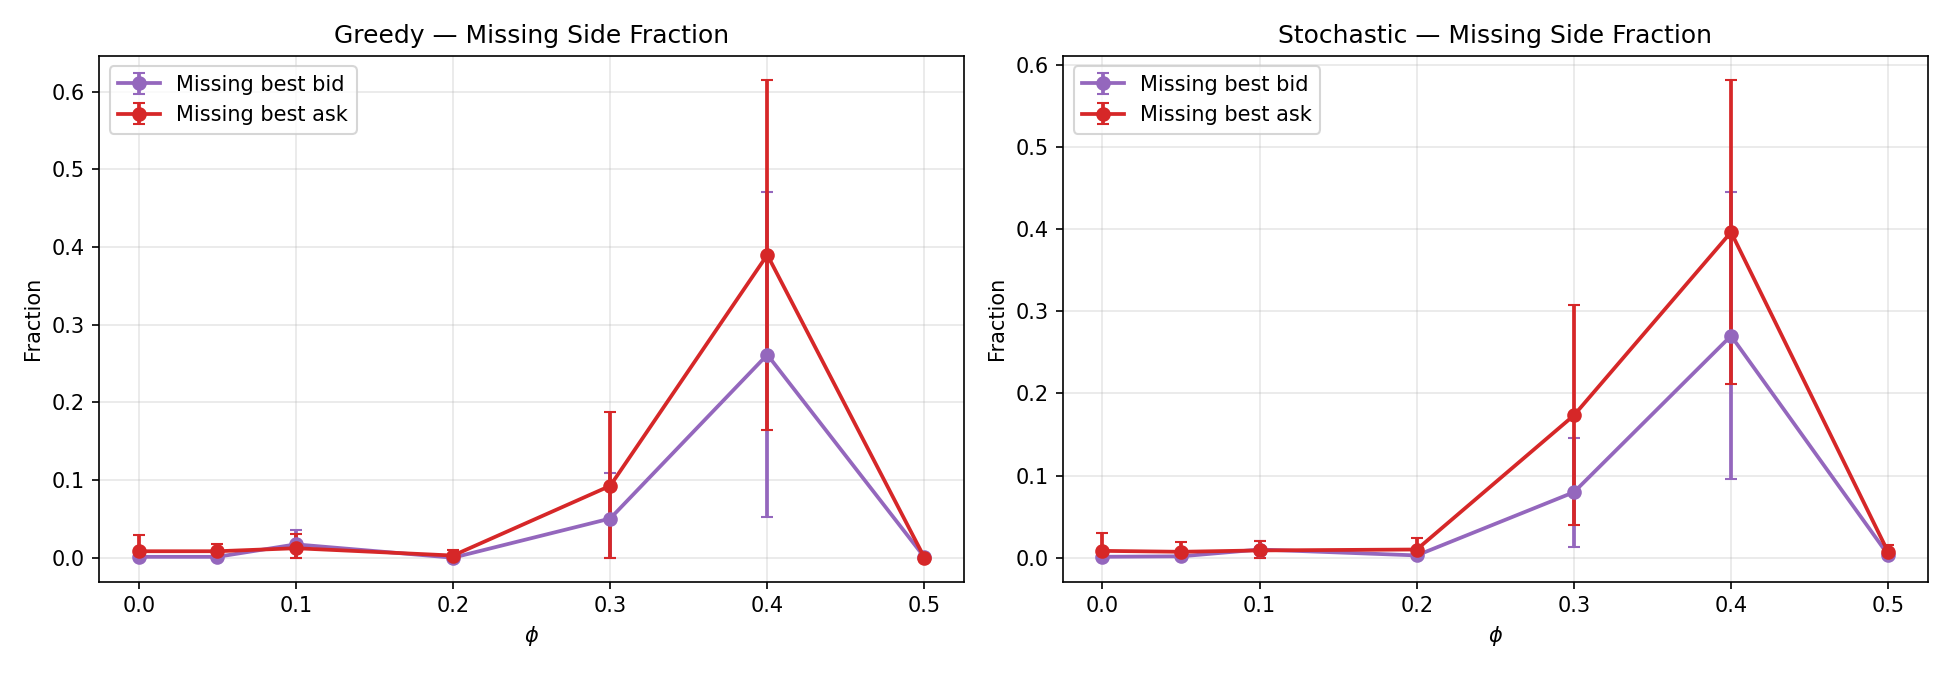
\includegraphics[width=\columnwidth]{figure_both_test.png}
    \caption{One-Sided Order Book Fraction vs $\phi$ by Liquidity Mode. Comparison between taker-only and mixed configurations.}
    \label{fig:liquidity-modes}
\end{figure}

\FloatBarrier

\subsection{Persistence of One-Sided States}

I next analyze the duration of one-sided states to determine whether these failures are transient or persistent.

As shown in Figure~\ref{fig:max-consecutive-duration}, the maximum consecutive duration of one-sided states increases significantly with $\phi$, particularly between $\phi = 0.3$ and $\phi = 0.4$. Figure~\ref{fig:p90-duration} shows the same pattern in the upper tail of episode duration. Taken together, these results indicate that once the system enters a one-sided state, recovery becomes increasingly difficult. 
\begin{figure}[htbp]
    \centering
    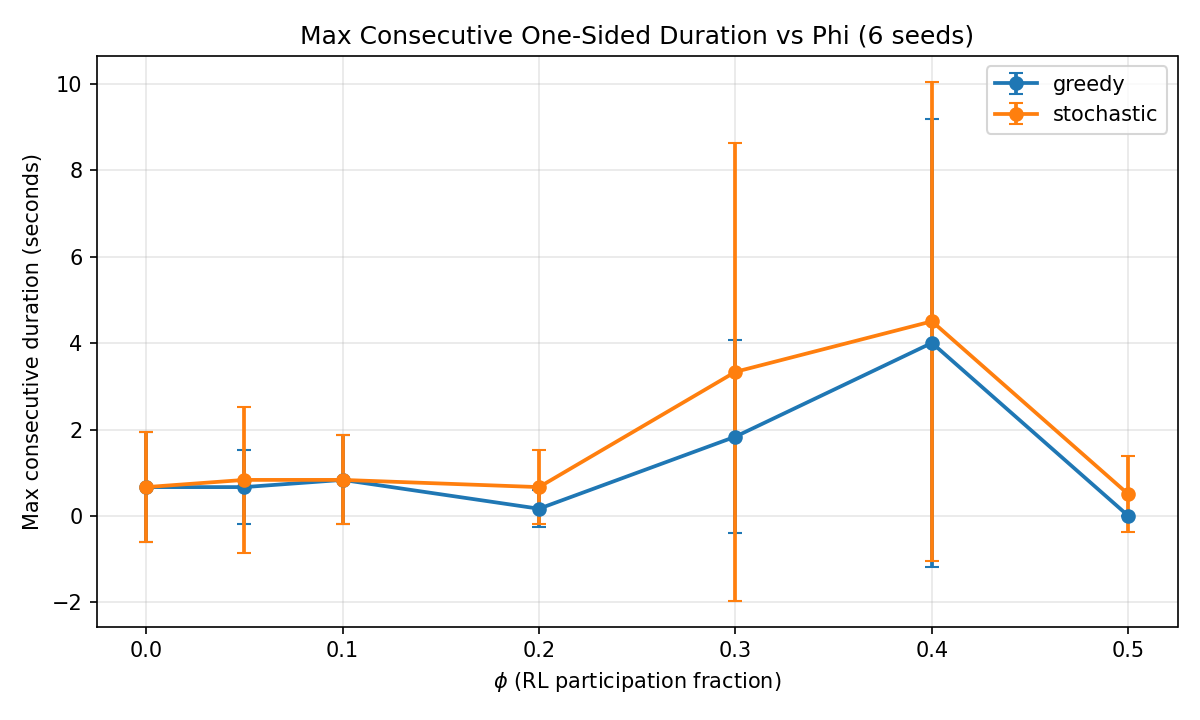
\includegraphics[width=\columnwidth]{max_consecutive_one_sided_duration_with_ci_vs_phi.png}
    \caption{Max Consecutive One-Sided Duration vs $\phi$. Maximum length of consecutive one-sided order book states observed during each simulation, with uncertainty shown across runs.}
    \label{fig:max-consecutive-duration}
\end{figure}
The failure is therefore not just more frequent at higher RL participation, but also more structurally persistent.



\begin{figure}[htbp]
    \centering
    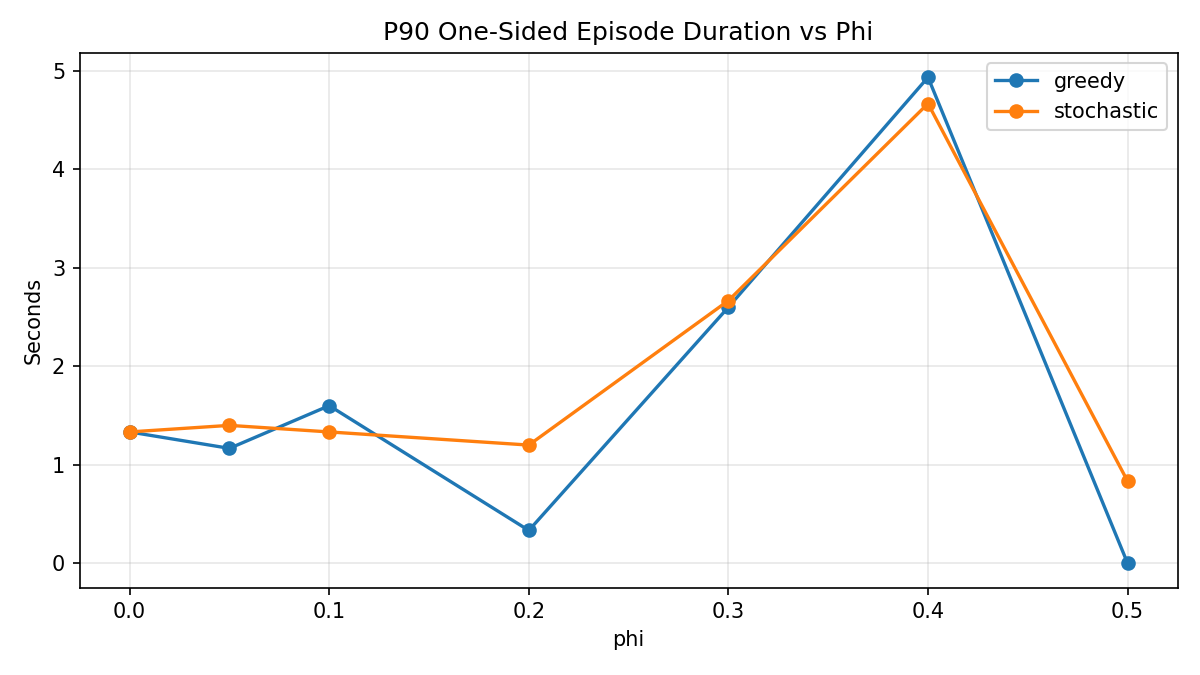
\includegraphics[width=\columnwidth]{figure4.png}
    \caption{P90 One-Sided Episode Duration vs $\phi$. 90th percentile duration of one-sided episodes, indicating the persistence of liquidity failures.}
    \label{fig:p90-duration}
\end{figure}

\FloatBarrier

\subsection{Mechanism}

To understand the mechanism behind these failures, I examine agent behavior through action distributions and inactivity rates.

Figure~\ref{fig:action-fractions} shows that action distributions shift with increasing $\phi$. Figure~\ref{fig:shutdown-support} and Figure~\ref{fig:inactivity-standalone} show that inactivity also rises, especially at $\phi = 0.5$. However, the most severe one-sided failures occur at intermediate values of $\phi$, where agents remain partially active. This matters because it separates the breakdown from a trivial policy collapse. The evidence suggests that the system fails not because agents stop participating altogether, but because they participate in an uneven way that drains one side of the book faster than it can be replenished.

At $\phi = 0.5$, inactivity approaches 100\%, indicating that agents largely cease interaction with the market. 
\begin{figure}[htbp]
    \centering
    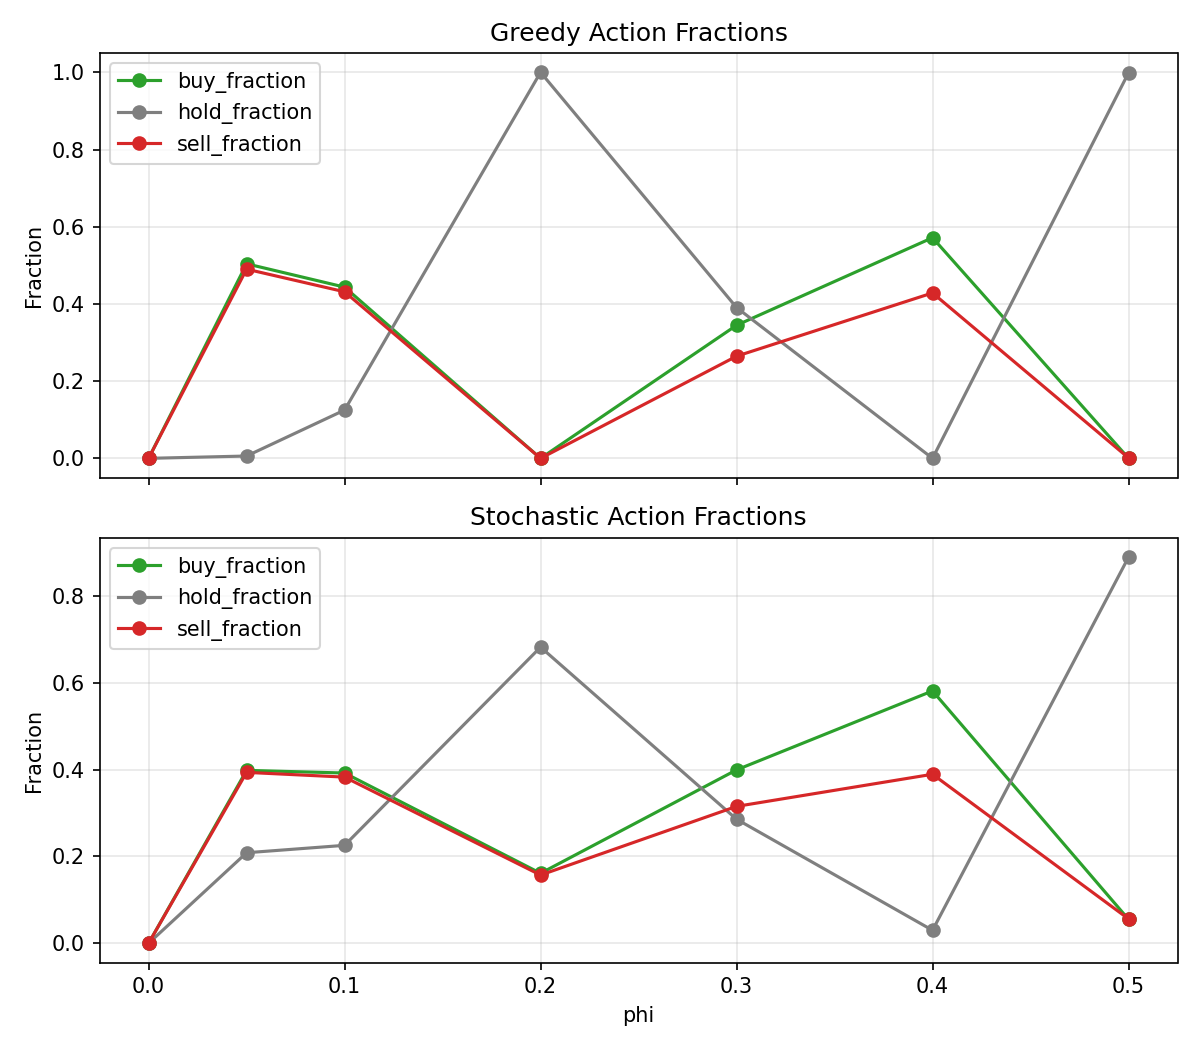
\includegraphics[width=\columnwidth]{figure5.png}
    \caption{RL Action Fractions vs $\phi$. Distributions of buy, sell, and hold actions for RL agents under greedy and stochastic evaluation modes.}
    \label{fig:action-fractions}
\end{figure}
This regime is better interpreted as market shutdown than as market recovery. The apparent improvement in one-sided-book metrics at this point reflects the disappearance of meaningful order flow rather than the restoration of balanced liquidity.



\begin{figure}[htbp]
    \centering
    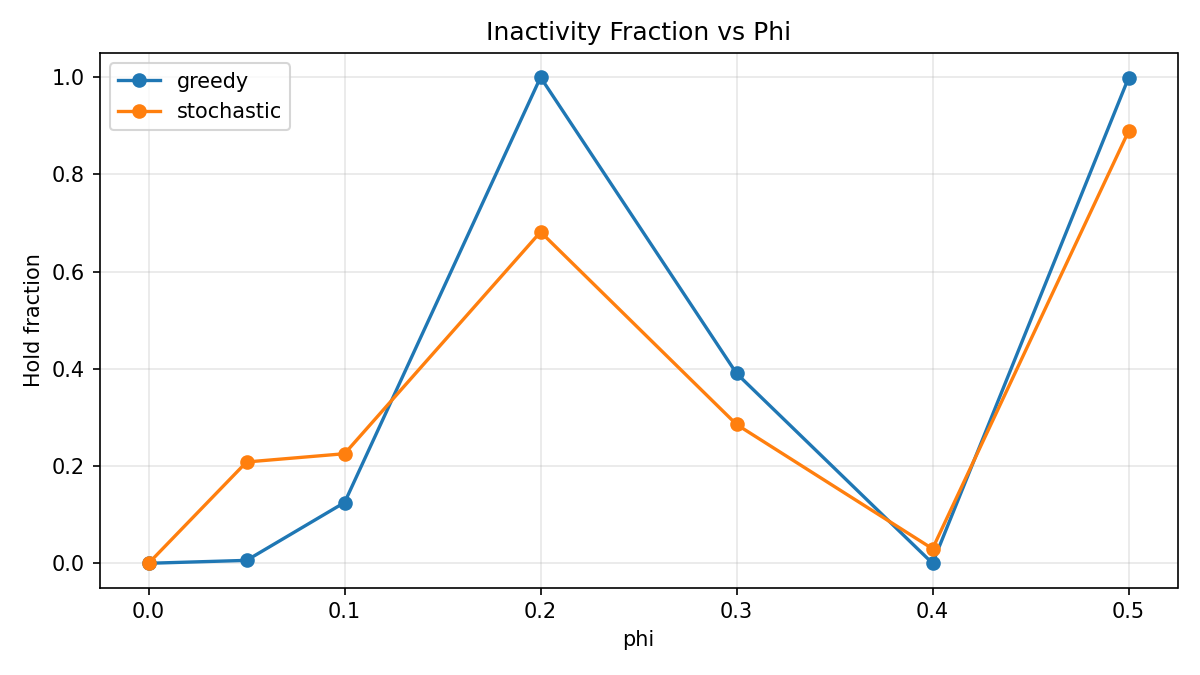
\includegraphics[width=\columnwidth]{figure6.png}
    \caption{Inactivity Fraction vs $\phi$. Fraction of timesteps in which agents select the hold action, indicating reduced participation.}
    \label{fig:inactivity-standalone}
\end{figure}

\FloatBarrier

\subsection{Analytical Threshold}

The mechanism described above suggests a simple mean-field prediction for the transition point. Let $C(\phi)$ denote the aggregate liquidity consumption rate and $P(\phi)$ denote the aggregate provision rate:
\begin{align*}
C(\phi) &= 80\phi \cdot \lambda_r \\
P(\phi) &= 80(1-\phi) \cdot \lambda_n + 2\lambda_m
\end{align*}
where $\lambda_r$ is the per-agent RL execution rate (market orders per second), $\lambda_n$ is the noise trader limit-order provision rate, and $\lambda_m$ is the market maker provision rate per maker.

From the simulation parameters, $\lambda_n = 0.09$ limit orders per second per noise trader (wake frequency $5\text{s}$, submission probability $0.45$) and $\lambda_m = 10$ units per second per market maker (wake frequency $1\text{s}$, quote size $5$, both sides). Estimating $\lambda_r$ empirically from pre-breakdown regimes ($\phi \in \{0.05, 0.10\}$) gives $\lambda_r \approx 1.06$ executed orders per second per agent.

Setting $C(\phi^*) = P(\phi^*)$ and solving:
\[
\phi^* = \frac{80\lambda_n + 2\lambda_m}{80(\lambda_n + \lambda_r)} \approx 0.30
\]

As shown in Figure~\ref{fig:threshold}, this predicted threshold aligns closely with the empirically observed transition: one-sided book failures remain low for $\phi \leq 0.20$ and spike sharply at $\phi = 0.30$, where $C(0.30) \approx P(0.30)$. At $\phi = 0.40$, consumption exceeds provision by nearly 40\%, consistent with the near-total one-sided failure observed at that level. The agreement between the simple flow-rate argument and the empirical data supports the interpretation that the failure is driven by the imbalance between RL liquidity consumption and the market's replenishment capacity.

\begin{figure}[htbp]
    \centering
    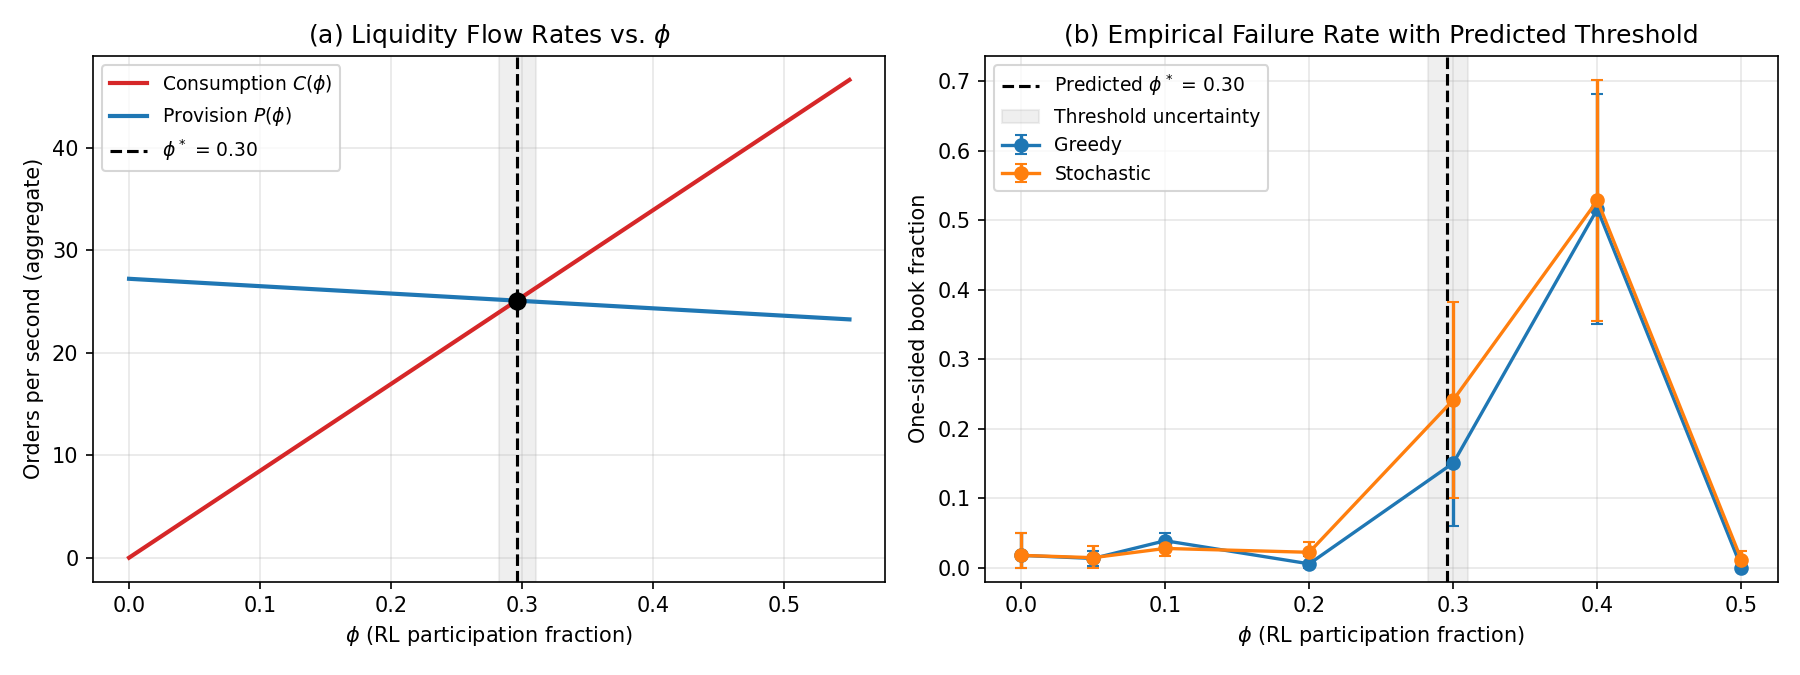
\includegraphics[width=\columnwidth]{threshold_analysis.png}
    \caption{Analytical threshold $\phi^*$ vs.\ empirical one-sided book fraction. Left: aggregate consumption rate $C(\phi)$ and provision rate $P(\phi)$ cross at $\phi^* \approx 0.30$ (shaded band shows uncertainty from $\lambda_r$ estimates). Right: empirical one-sided fraction with the predicted threshold overlaid; the sharp empirical rise aligns with the crossing point.}
    \label{fig:threshold}
\end{figure}

\FloatBarrier

\subsection{Effects of Inventory Constraints}

To evaluate the role of inventory exposure, I introduce inventory constraints and repeat the $\phi$-sweep.

As shown in Figure~\ref{fig:inventory-cap-frequency}, adding an inventory constraint significantly reduces the frequency of one-sided states across all values of $\phi$. Figure~\ref{fig:inventory-cap-duration} shows that the same intervention also shortens the duration of breakdown episodes. This suggests that inventory risk is not just correlated with the failure, but is central to sustaining it. When agents are prevented from accumulating large directional positions, their ability to continue draining one side of the book is reduced, and the system becomes meaningfully more stable.

\begin{figure}[htbp]
    \centering
    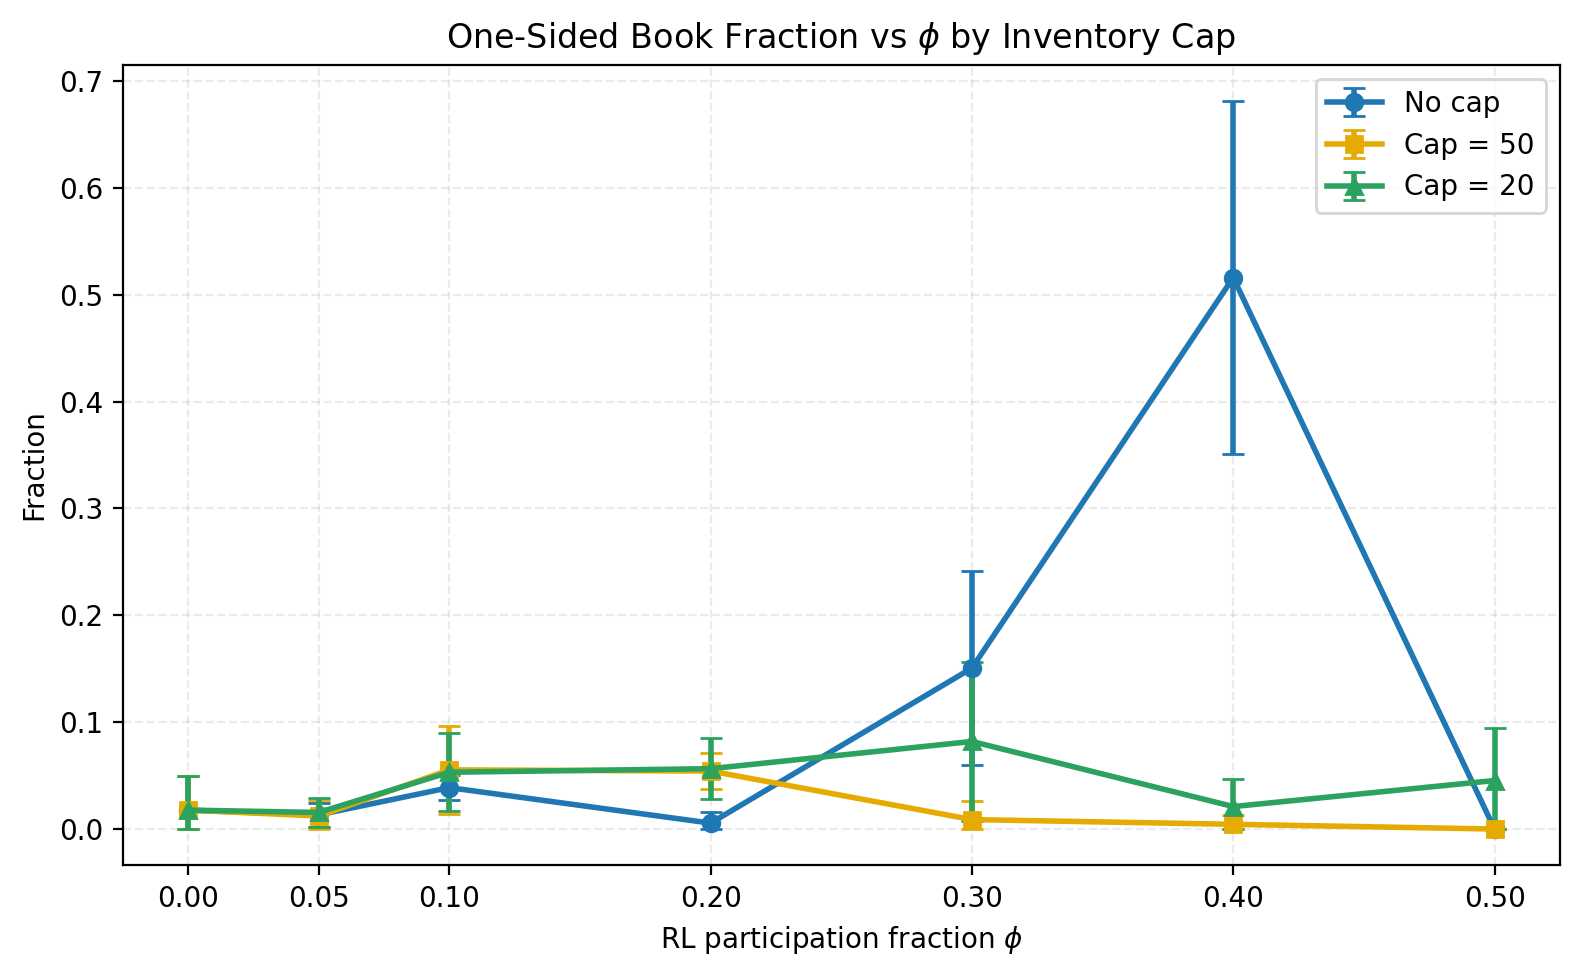
\includegraphics[width=\columnwidth]{inventory_cap_one_sided_fraction_with_ci_vs_phi.png}
    \caption{One-Sided Order Book Fraction vs $\phi$ by Inventory Cap. Comparison of one-sided order book frequency under different inventory constraint levels, with uncertainty shown across runs.}
    \label{fig:inventory-cap-frequency}
\end{figure}

\begin{figure}[htbp]
    \centering
    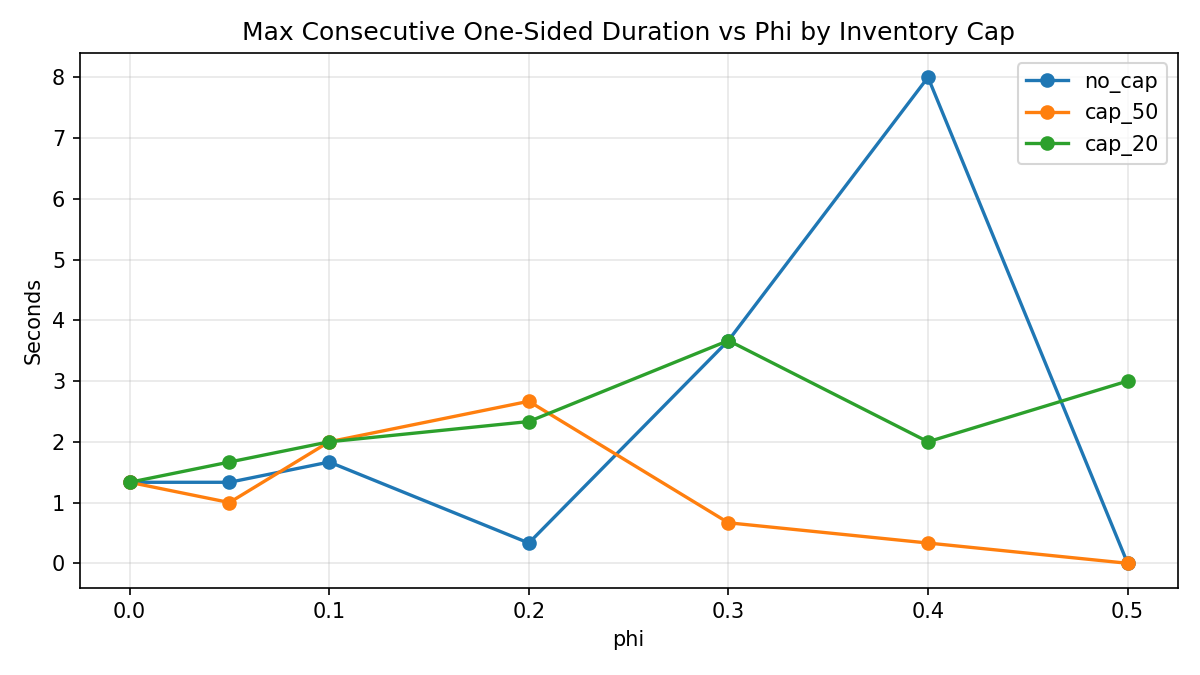
\includegraphics[width=\columnwidth]{figure10.png}
    \caption{Max Consecutive One-Sided Duration vs $\phi$ by Inventory Cap. Maximum duration of one-sided states under different inventory constraint levels.}
    \label{fig:inventory-cap-duration}
\end{figure}

These results indicate that inventory risk plays a central role in the observed liquidity withdrawal behavior.

\FloatBarrier

\subsection{Trained Policies vs Random Baseline}

To determine whether the observed effects arise from learned behavior, I compare trained RL agents with a random baseline policy.

As shown in Figure~\ref{fig:policy-type}, the random baseline exhibits a smoother and more monotonic increase in one-sided states as $\phi$ increases. In contrast, the trained policy produces a sharper, nonlinear spike, particularly at $\phi = 0.4$. This difference suggests that the breakdown is not simply a consequence of replacing noise traders with arbitrary agents. Instead, the learned policy introduces a more concentrated and destabilizing form of participation that is not reproduced by random action selection alone.

\begin{figure}[htbp]
    \centering
    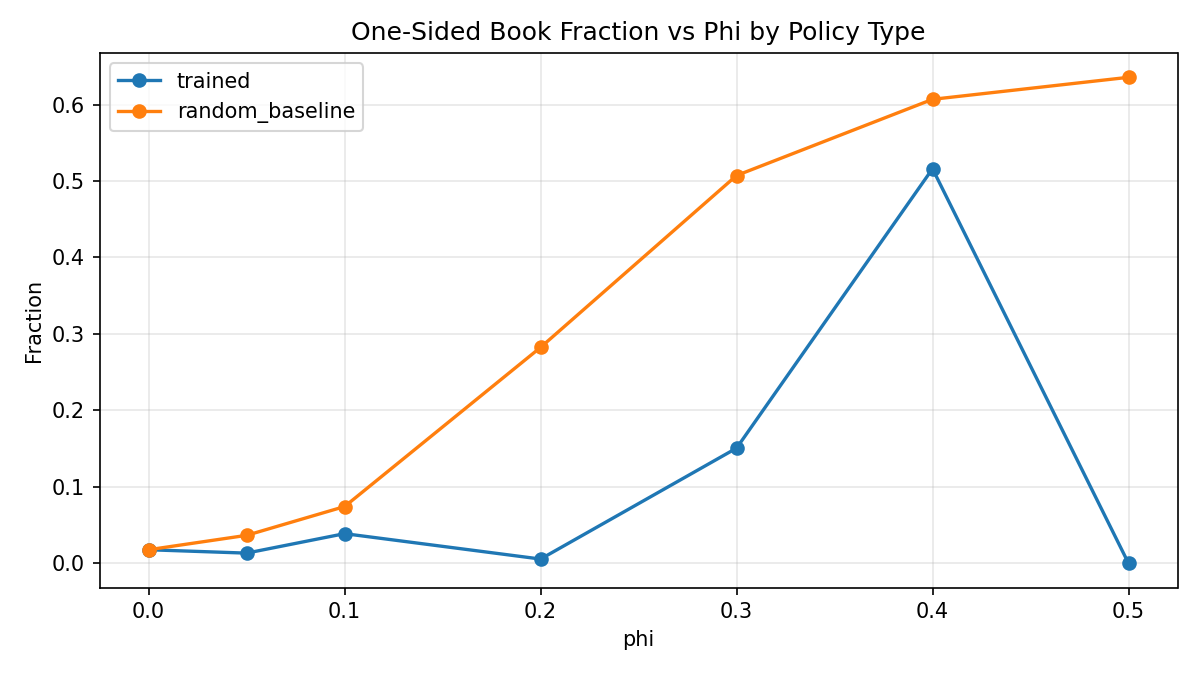
\includegraphics[width=\columnwidth]{figure11.png}
    \caption{One-Sided Order Book Fraction vs $\phi$ by Policy Type. Comparison between trained RL policies and random baseline agents.}
    \label{fig:policy-type}
\end{figure}

\FloatBarrier

\subsection{Summary of Findings}

Across all experiments, I observe a consistent pattern. Increasing RL participation leads to a nonlinear rise in one-sided order book states, with the strongest effects occurring at intermediate values of $\phi$. These states become persistent, indicating sustained breakdowns in liquidity rather than transient imbalances.

The results suggest that the core failure is a breakdown in balanced participation rather than a simple increase in inactivity. At very high levels of RL participation, the system transitions into a degenerate regime characterized by near-total inactivity. This suppresses failures in the narrow sense measured by one-sided-book frequency, but only because meaningful trading largely disappears. Importantly, these failures persist even when RL agents are allowed to provide passive liquidity, indicating that the effect is not solely driven by the absence of liquidity provision.

Inventory constraints significantly mitigate both the frequency and persistence of one-sided states, demonstrating that inventory caps are a key driver of the observed behavior. Additionally, the effect is specific to learned policies and not reproduced by random baselines.

Together, these findings support the existence of an endogenous failure mode in which learned trading behavior degrades liquidity by altering participation in the limit order book.

\section{Discussion}

The main result of this paper is that increasing the participation of learned trading agents can produce persistent one-sided order book states in a limit order book environment. These failures are not well described by changes in volatility or spread alone. Instead, the core failure is structural: one side of the top of the book disappears, and mid-price formation becomes undefined.

Importantly, these failures persist even when reinforcement learning agents are allowed to provide passive liquidity. While enabling quoting behavior reduces the severity of one-sided states, it does not eliminate them. This rules out a purely mechanical explanation based on the removal of liquidity-providing agents and instead suggests that learned behavior itself alters participation in a way that can destabilize the order book.

This distinguishes the present results from much of the reinforcement learning literature in trading. Prior work has focused on optimizing execution, inventory control, or market making performance at the level of individual agents (Spooner et al., 2018; Nevmyvaka et al., 2006). These approaches often rely on historical replay or assume negligible market impact, limiting their ability to capture system-level effects that arise when multiple adaptive agents interact (Balch et al., 2019). As a result, they do not address how learned behavior alters the structure of the market itself.

The broader idea that agent behavior can degrade liquidity is well established in agent-based modeling. Prior work has shown that interactions between heterogeneous traders can generate endogenous instability, particularly through coordination effects such as herding (Lussange et al., 2024). However, these mechanisms are typically driven by imitation or correlated behavior. In contrast, the results here are more consistent with uneven participation and selective liquidity withdrawal emerging from learned policies.

A simple flow-rate argument provides a theoretical basis for the observed threshold. When RL agents consume liquidity faster than noise traders and market makers can replenish it, one-sided states become persistent. Solving for the breakeven fraction yields $\phi^* \approx 0.30$, which aligns with the empirical transition observed in the data. This connection between the micro-level parameters of agent behavior and a macro-level market failure condition strengthens the interpretation that the breakdown is mechanistically driven rather than coincidental.

The contribution of this paper is therefore more specific. First, it identifies a structural failure mode at the level of the top of the order book, rather than relying on aggregate measures such as volatility or trading volume. Second, it shows that this failure emerges as a function of the fraction of learning-based agents, $\phi$, exhibiting a nonlinear transition at intermediate values of $\phi$. Third, it demonstrates that this effect persists even when learning agents provide liquidity, indicating that the failure is not solely due to the removal of passive orders. Finally, it identifies inventory constraints as an effective mitigation mechanism that reduces both the frequency and persistence of these failures.

The role of inventory constraints is particularly important. In the unconstrained setting, agents can accumulate positions that expose them to risk, which may lead to reduced participation or asymmetric behavior. When inventory caps are introduced, both the frequency and persistence of one-sided states are significantly reduced. This suggests that inventory risk is a key driver of the observed liquidity withdrawal behavior. This interpretation is also consistent with classical market-making models such as Avellaneda and Stoikov (2008), where inventory control is central to maintaining stable quoting behavior.

The shutdown evidence at $\phi = 0.5$ further clarifies the mechanism. As shown in Figure~\ref{fig:shutdown-support}, the drop in one-sided failures at this point coincides with sharply increased inactivity and zero-return behavior plus sharply reduced quote activity. This means the system is not recovering stable two-sided liquidity at $\phi = 0.5$. Instead, it is moving into a degenerate regime with very little meaningful market activity. This distinction matters because it shows that lower failure frequency does not necessarily imply a healthier market state.

The comparison with the random baseline reinforces this interpretation. The random baseline produces a smoother and more monotonic degradation in market quality, whereas the trained policy generates a sharper and more concentrated spike in one-sided states. This indicates that the observed failure mode arises from the structure of learned policies rather than from the mere presence of additional agents.

These findings should be interpreted with appropriate caution. The experiments are conducted in a single ABIDES-based simulation environment (Byrd et al., 2020) and rely on a specific RL training setup. As a result, the paper does not claim that these effects represent a universal property of financial markets. Instead, it identifies a reproducible failure mode within a realistic and widely used simulation framework. ABIDES is designed to capture detailed market microstructure and agent interaction, but results obtained in simulation do not automatically generalize to real-world markets.

Overall, these results highlight an important implication. Learned trading agents should not be evaluated solely on individual performance metrics. A policy that appears effective in isolation may still degrade market quality when deployed alongside other adaptive agents. This suggests that system-level effects are critical for evaluating learning-based trading systems and that such systems may introduce new forms of instability when scaled.

\section{Limitations}

\subsection{Simulation Environment}

The primary results of this paper are obtained within the ABIDES platform (Byrd et al., 2020) using a fixed RMSC04-style configuration. As a robustness check, I evaluate the same phi-sweep under an alternative market ecology (ZIC traders as the dominant flow provider with fifteen market makers rather than two). Under this alternative configuration, no one-sided order book failures are observed across any value of $\phi$ up to 0.60 (Figure~\ref{fig:alt-profile-comparison}). At most $\phi$ values, RL agents converge to symmetric alternating buy/sell strategies or fully passive hold policies, neither of which creates the persistent one-sided pressure observed in the primary setting. This null result is consistent with the theoretical threshold $\phi^*$, which explicitly depends on the market maker arrival rate $\lambda_m$: with fifteen times as many market makers, the provision rate $P(\phi)$ is substantially higher, pushing $\phi^*$ far beyond what is achievable within the simulation. The failure mode identified in the primary experiment is therefore contingent on limited market maker coverage, not an artifact of any single aspect of the simulation design.

\begin{figure}[htbp]
    \centering
    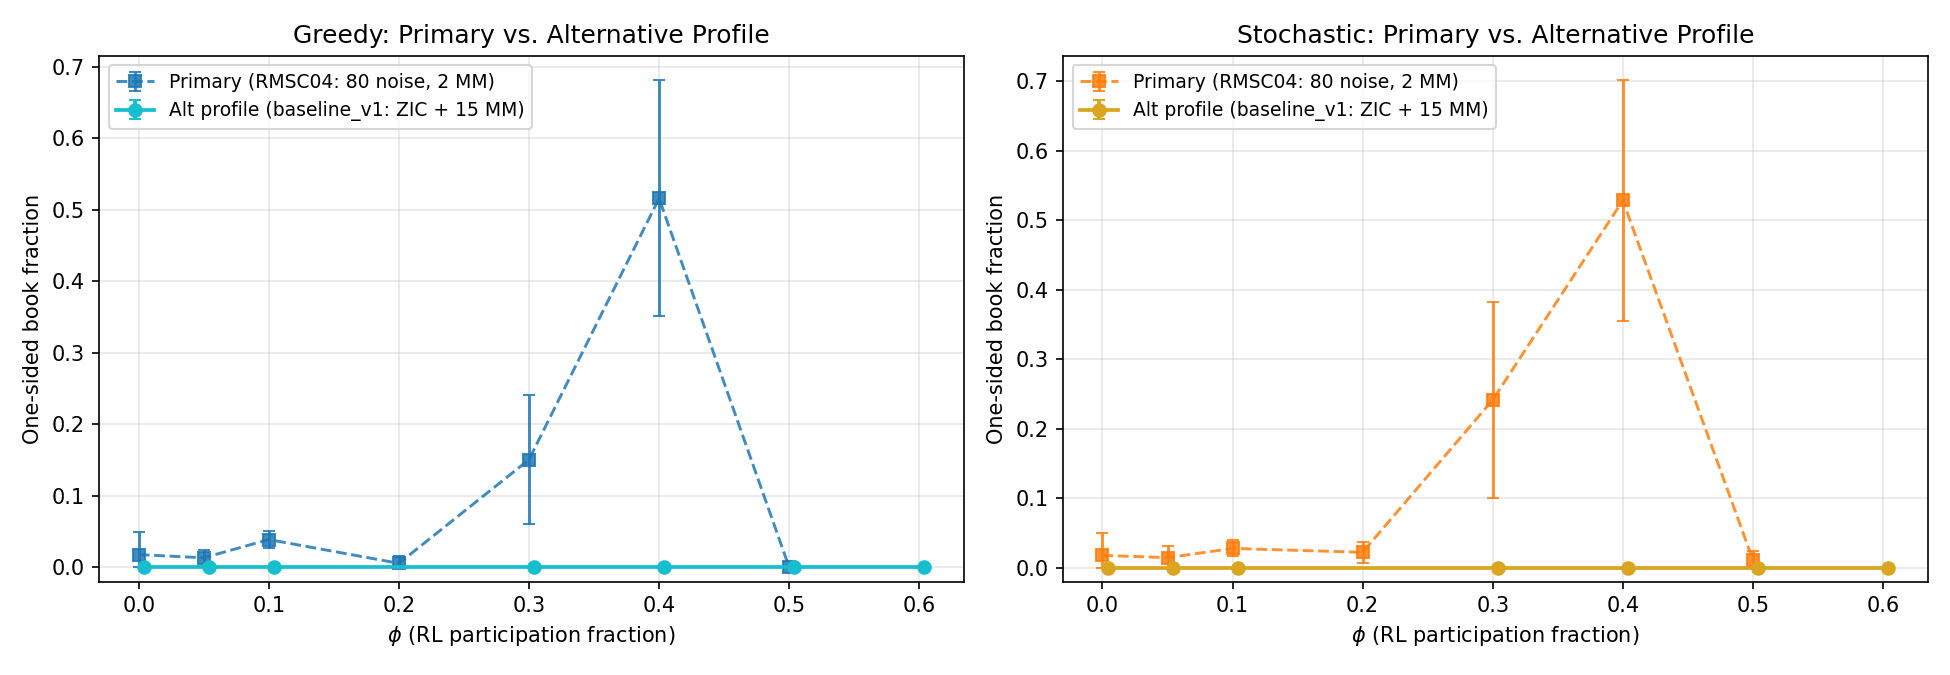
\includegraphics[width=\columnwidth]{alt_profile_comparison.png}
    \caption{Alternative Market Profile Robustness Check. One-sided book fraction vs $\phi$ under the primary configuration (RMSC04: 80 noise traders, 2 market makers) and the alternative configuration (ZIC: 51 ZIC traders, 15 market makers). The alternative profile produces zero one-sided failures across all $\phi$ values, demonstrating that the failure mode depends on limited market maker coverage.}
    \label{fig:alt-profile-comparison}
\end{figure}

The agent population, matching rules, and oracle dynamics are specified by the simulation design. In particular, the latent fundamental value follows a simple stochastic process, and agent behaviors are limited to predefined classes. As a result, the findings should be interpreted as demonstrating a reproducible failure mode within this framework, rather than a universal property of real-world markets.

\subsection{Restricted Agent Behavior}

A structural limitation of the current setup is that RL agents do not uniformly provide passive liquidity across all configurations. While the baseline setup consists of agents that primarily consume liquidity through market orders, additional experiments introduce agents that submit passive limit quotes. However, these quoting behaviors are simplified and do not fully capture realistic market-making strategies.

This design choice affects how the results should be interpreted. Increasing $\phi$ replaces liquidity-providing noise traders with agents whose behavior differs in both execution and participation. As a result, part of the observed degradation in market structure reflects a shift in market composition.

However, the observed effects are not consistent with a purely mechanical replacement story. In particular, the nonlinear spike in one-sided order book states at intermediate values of $\phi$, along with differences between trained policies and random baselines, indicate that learned behavior plays a central role in shaping market outcomes.

Nonetheless, the current setup only considers simplified forms of passive liquidity provision and does not capture more sophisticated market-making strategies. Future work should extend the analysis to richer quoting behaviors and adaptive liquidity provision mechanisms.

\subsection{Policy and Reward Design Dependence}

The learned behavior depends directly on the reward function and training configuration. In this work, the reward includes marked-to-market wealth changes, inventory penalties, and optional inactivity penalties. Different reward specifications or hyperparameter choices could produce qualitatively different agent behavior.

In particular, the emergence of inactivity at high values of $\phi$ suggests that the learned policy can converge to degenerate strategies characterized by near-total inactivity under certain conditions. Although anti-degeneracy penalties reduce this effect, they do not eliminate it entirely. This indicates that the observed dynamics are sensitive to policy design and should not be interpreted as invariant across all RL formulations.

\subsection{Limited Exploration of Parameter Space}

The experiments focus on a fixed market configuration with a specific agent composition and a discrete set of $\phi$ values. While the results show consistent behavior across this grid, they do not establish robustness across alternative environments or broader regions of the parameter space.

In particular, the results are based on replacing noise traders with RL agents, while keeping value traders and market makers fixed. Different replacement schemes or alternative baseline populations could lead to different outcomes. Similarly, the analysis does not explore sensitivity to key parameters such as order size, time horizon, or market volatility.

\subsection{Interpretation of One-Sided States}

The definition of one-sided order book states is based on the absence of the best bid or best ask in logged top-of-book snapshots. While this provides a clear and measurable failure condition, it is a relatively strict definition.

In real markets, liquidity may degrade without completely disappearing from one side of the book. Therefore, the results should be interpreted as capturing a severe form of liquidity failure, rather than the full spectrum of market degradation.

\subsection{External Validity and Real-World Implications}

These findings do not imply that real financial systems will exhibit identical behavior under the introduction of RL-based trading systems. Real markets include additional structure, such as regulatory constraints, diverse participant objectives, and institutional risk management systems, which are not fully captured in the simulation.

However, the results are consistent with broader concerns in the literature that algorithmic and AI-driven trading systems may contribute to liquidity withdrawal under certain conditions (IMF, 2023). The contributions of this work are therefore best understood as identifying a plausible mechanism for liquidity breakdown in learning-based markets that warrants further investigation, rather than making direct claims about real-world market outcomes.

\section{Conclusion}

This paper studies how increasing the participation of reinforcement learning (RL) agents affects liquidity in a limit order book. Using an agent-based market simulation, I vary the fraction of RL agents, $\phi$, and analyze the resulting changes in market structure.

I find that increasing RL participation leads to a nonlinear rise in persistent one-sided order book states, where one side of the book disappears and price information becomes undefined. These failures are most pronounced at intermediate values of $\phi$ and are characterized by sustained periods of missing liquidity rather than short-lived imbalances.

Importantly, these effects are not solely driven by trivial inactivity or by the absence of liquidity provision. Even when RL agents are allowed to submit passive limit quotes, one-sided order book states persist, although their severity is reduced. This indicates that the observed breakdown is not purely mechanical, but instead arises from changes in participation behavior induced by learned policies.

I also show that inventory constraints significantly reduce both the frequency and persistence of one-sided states. This highlights the role of inventory exposure in shaping agent behavior and suggests that simple structural constraints can mitigate the impact of learning-based trading strategies on market stability.

The evidence at $\phi = 0.5$ further shows that a reduction in one-sided-book failures does not necessarily imply improved liquidity. In this regime, failures decline because market participation largely collapses, not because the market recovers healthy two-sided trading.

Overall, the results identify a failure mode in which learned trading behavior degrades liquidity at the level of market structure. This suggests that evaluating trading agents solely on individual performance is insufficient, and that system-level effects must be considered when designing and deploying learning-based trading systems.

Future work should extend this analysis to settings in which agents jointly learn both liquidity provision and inventory management, as well as to alternative market environments and agent compositions.

\section*{References}

\begin{itemize}[leftmargin=2em]
    \item Nevmyvaka et al., 2006 - Reinforcement Learning for Optimized Trade Execution (\url{https://www.cis.upenn.edu/~mkearns/papers/rlexec.pdf})

    \item Spooner et al., 2018 - Market Making via Reinforcement Learning (AAMAS) (\url{https://livrepository.liverpool.ac.uk/3020822/1/MM_aamas.pdf?utm})

    \item Balch et al., 2019 - How to Evaluate Trading Strategies: Single Agent Market Replay or Multiple Agent Interactive Simulation? (\url{https://www.jpmorgan.com/content/dam/jpm/cib/complex/content/technology/ai-research-publications/pdf-12.pdf?utm})

    \item Lussange et al., 2024 - Learning Behaviors and Mesoscale Effects in Multi-Agent Market Simulation (PLOS One) (\url{https://journals.plos.org/plosone/article?id=10.1371\%2Fjournal.pone.0301141&utm})

    \item Farmer \& Foley, 2009 - The Economy Needs Agent-Based Modelling (Nature) (\url{https://www.inet.ox.ac.uk/publications/the-economy-needs-agent-based-modelling})

    \item Bank of England, 2020 - The Deeds of Speed: An Agent-Based Model of Market Liquidity and Flash Episodes (\url{https://www.bankofengland.co.uk/-/media/boe/files/working-paper/2018/the-deeds-of-speed-an-agent-based-model-of-market-liquidity-and-flash-episodes.pdf?utm})

    \item IMF, 2023 - Global Financial Stability Report -- AI and Financial Stability (\url{https://www.imf.org/en/publications/gfsr/issues/2023/10/10/global-financial-stability-report-october-2023?utm})

    \item Byrd et al., 2020 - ABIDES: Towards High-Fidelity Market Simulation for AI Research (\url{https://par.nsf.gov/servlets/purl/10185795})

    \item Avellaneda \& Stoikov, 2008 - High-Frequency Trading in a Limit Order Book (\url{https://people.orie.cornell.edu/sfs33/LimitOrderBook.pdf?utm})
\end{itemize}

\end{document}